\documentclass{hbrs-ecta-report}

\usepackage{float}
\usepackage{placeins}
\usepackage{ngerman}
\usepackage[utf8]{inputenc}
\begin{document}

\conferenceinfo{H-BRS}{2017}

\title{Neuroevolution: Simple Hill Climbing}
\subtitle{}

\numberofauthors{2}
\author{
\alignauthor
Tim L"ugger, Jan Urfei
}

\date{today}
\maketitle
\begin{abstract}
Aufgabe: Implementiere den HillClimb Algorithmus aus der Vorlesung und f"uhre diesen 100 Mal mit einer vorgegebenen Kostenfunktion aus.
\end{abstract}

\section{Der HillClimb Algorithmus}
Der HillClimb Algorithmus ben"otigt eine Kostenfunktion, anhand derer das Ergebnis bewertet wird, um eine möglichst optimale L"osung zu finden. Zuerst wird ein zuf"alliger Wert generiert von dem aus benachbarte Werte gewählt werden. Für diese werte wird die 'Fitness' bestimmt indem sie in die Kostenfunktion eingesetzt werden. Man wählt nun den Wert mit der größten Fitness von dem erneut Nachbarn gebildet werden. Der Algorithmus endet entweder nach einer festen Anzahl an Iterationen oder wenn sich das Ergebnis nicht mehr "andert.

\section{Herangehensweise}

Es wird ein zufälliger Startwert $x$ zwischen $0$ und $2$ gewählt. Als Nachbarn gilt immer $x - 0.1$ und $x + 0.1$. Diese drei Werte werden in die Funktion fit(x) (Figure \ref{fig:fit}) eingesetzt. Der x-wert mit dem größten fit(x) wird als nächster Startwert verwendet. Dieser Vorgang wird 100 mal wiederholt. Der Startwert nach der letzten Iteration ist unsere Lösung. 



\section{Unsere Ergebnisse}
Die Fähigkeit dieses Verfahrens einen möglichst maximales fit(x) zu finden hängt besonders von der Wahl des zufälligen Startwertes ab, da für $x\leq1$ der Algorithmus im lokalen Maximum bei $x=0.5$ endet(Figure \ref{fig:fit_local_max_right} und Figure \ref{fig:fit_local_max_left}). Da fit(x) für alle $x>1$ streng monoton wachsend ist, steigt der gewählte x-wert 
an, bis das Iterationslimit erreicht ist (Figure \ref{fig:fit_max}). 
Da das Maximum davon abhängt, ob der Startwert größer als 1 ist oder nicht und das genau die Mitte des Intervalls ist, in dem der Startwert gebildet wird ist auch die Verteilung der Zwei Maxima annähernd 50:50. Sehr gut kann man das in dem Histogramm beobachten (Figure \ref{fig:histogram}). Es wird sehr deutlich, das es zwei Gruppen an Lösungen gibt. Die, die bei 0.5 liegen und die, die größer 10.5 sind. Dadurch ist im Boxplot (Figure \ref{fig:boxplot}) der Bereich zwischen dem oberen und dem unteren Quartil sehr groß.


\section{plots}

\begin{figure}[ht!]
	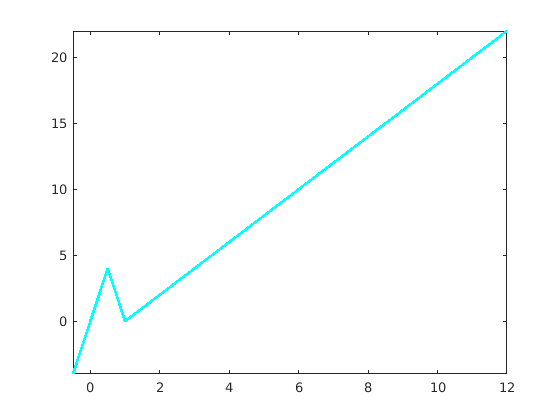
\includegraphics[width=\linewidth]{img/fit}
	\caption{Kostenfunktion: $fit(x) = (x>1).*(2.*x-2) + (x<=0.5).*8.*x + ((x>0.5).*(x<=1)).*(-8.*x + 8) $}
	\label{fig:fit}
\end{figure}
\begin{figure}[ht!]
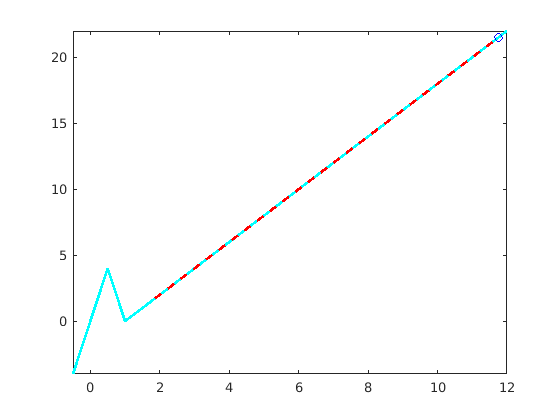
\includegraphics[width=\linewidth]{img/plot_fit_max.png}
\caption{$fit(Startwerte)$ aller Iterationen (rot), Maximum \small(blauer Kreis)}
\label{fig:fit_max} 
\end{figure}

\begin{figure}[t]
	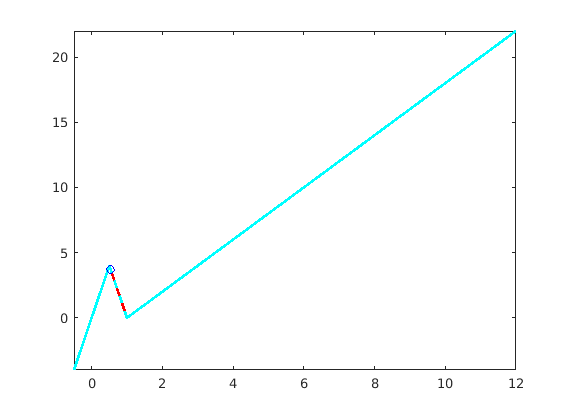
\includegraphics[width=\linewidth]{img/plot_fit_local_max_right.png}
	\caption{Lokales Maximum bei Startwert  $0.5 \leq x\leq1$ }
	\label{fig:fit_local_max_right} 
\end{figure}

\begin{figure}[t]
	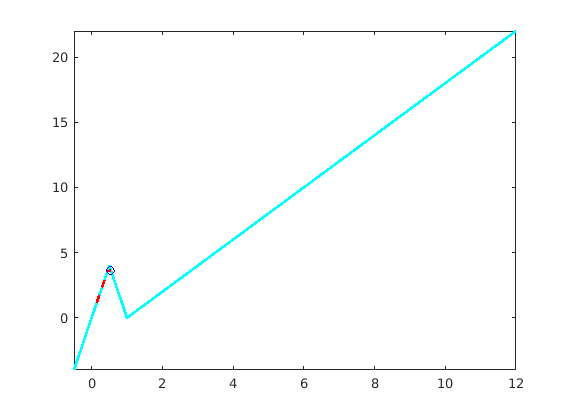
\includegraphics[width=\linewidth]{img/plot_fit_local_max_left.png}
	\caption{Lokales Maximum bei Startwert  $0.5 > x\leq1$ }
	\label{fig:fit_local_max_left} 
\end{figure}
\begin{figure}[p]
	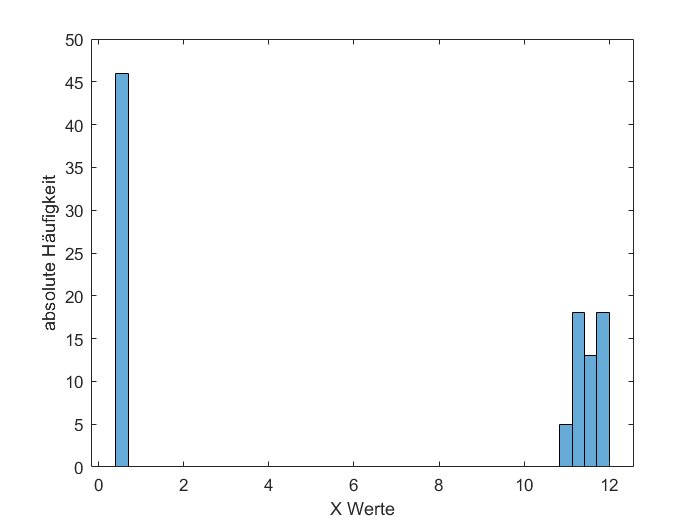
\includegraphics[width=\linewidth]{img/histogram_of_100_HillClimbs.png}
	\caption{Häufigkeitsverteilung der Maximalen x-Werte nach 100 fachem ausführen des HillClimb Algorithmus}
	\label{fig:histogram} 
\end{figure}
\begin{figure}[p]
	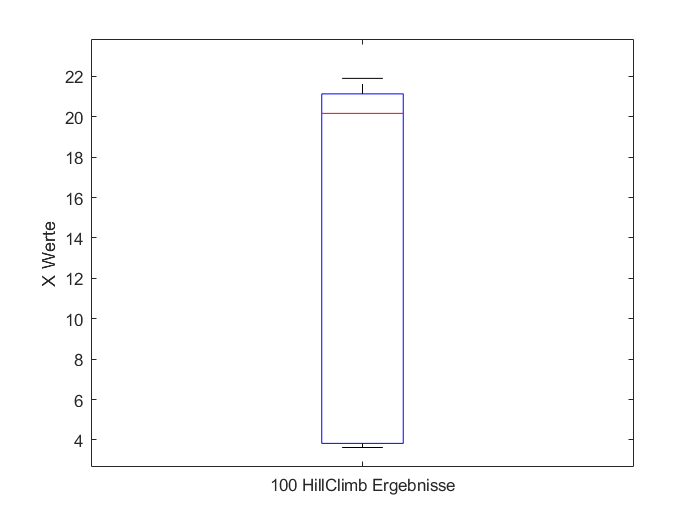
\includegraphics[width=\linewidth]{img/Boxplot_of_100HillClimbs.png}
	\caption{Häufigkeitsverteilung der Maximalen x-Werte nach 100 fachem ausführen des HillClimb Algorithmus}
	\label{fig:boxplot} 
\end{figure}


\end{document}
}